\documentclass[article]{report} % a4paper
% Some basic packages

\usepackage[utf8]{inputenc}
\usepackage[T1]{fontenc}
\usepackage{textcomp}
% Figure out whether you need this in English 
\usepackage[UKenglish]{babel}
\usepackage{url}
\usepackage{graphicx}
\usepackage{float}
\usepackage{booktabs}
\usepackage{enumitem}

% Don't indent paragraphs, leave some space between them
\usepackage{parskip}

% Hide page number when page is empty
\usepackage{emptypage}
\usepackage{subcaption}
\usepackage{multicol}
\usepackage{xcolor}

% Other font I sometimes use.
% \usepackage{cmbright}

% Math stuff
\usepackage{amsmath, amsfonts, mathtools, amsthm, amssymb}
% \usepackage{physics}
% Fancy script capitals
\usepackage{mathrsfs}
\usepackage{cancel}
% Bold math
\usepackage{bm}
% Some shortcuts
\newcommand\N{\ensuremath{\mathbb{N}}}
\newcommand\R{\ensuremath{\mathbb{R}}}
\newcommand\Z{\ensuremath{\mathbb{Z}}}
\renewcommand\O{\ensuremath{\emptyset}}
\newcommand\Q{\ensuremath{\mathbb{Q}}}
\newcommand\C{\ensuremath{\mathbb{C}}}
\newcommand\T{\ensuremath{\mathbb{T}}}
\newcommand\U{\ensuremath{\mathscr{U}}}
\newcommand\Y{\ensuremath{\mathscr{Y}}}
\newcommand\F{\ensuremath{\mathbb{F}}}

\newcommand{\norm}[1]{\left\lVert#1\right\rVert}
\let\newforall\forall
\renewcommand\forall{\;\newforall\;}
% Put x \to \infty below \lim
\let\svlim\lim\def\lim{\svlim\limits}

%Make implies and impliedby shorter
\let\implies\Rightarrow
\let\impliedby\Leftarrow
\let\iff\Leftrightarrow
\let\epsilon\varepsilon

% Add \contra symbol to denote contradiction
\usepackage{stmaryrd} % for \lightning
\newcommand\contra{\scalebox{1.5}{$\lightning$}}

% \let\phi\varphi

% Command for short corrections
% Usage: 1+1=\correct{3}{2}

\definecolor{correct}{HTML}{009900}
\newcommand\correct[2]{\ensuremath{\:}{\color{red}{#1}}\ensuremath{\to }{\color{correct}{#2}}\ensuremath{\:}}
\newcommand\green[1]{{\color{correct}{#1}}}

% horizontal rule
\newcommand\hr{
    \noindent\rule[0.5ex]{\linewidth}{0.5pt}
}

% hide parts
\newcommand\hide[1]{}

% si unitx
\usepackage{siunitx}
\sisetup{locale = FR}

% Environments
\makeatother
% For box around Definition, Theorem, \ldots
\usepackage{mdframed}
\mdfsetup{skipabove=1em,skipbelow=0em}
\theoremstyle{definition}
\newmdtheoremenv[nobreak=true]{consequence}{Consequence}
\newmdtheoremenv[nobreak=true]{theorem}{Theorem}
\newmdtheoremenv[nobreak=true]{lemma}{Lemma}
\newmdtheoremenv[nobreak=true]{definition}{Definition}
\newmdtheoremenv[nobreak=true]{prop}{Proposition}
\newmdtheoremenv[nobreak=true]{law}{Law}
\newmdtheoremenv[nobreak=true]{corollary}{Corollary}
\newmdtheoremenv{conclusion}{Conclusion}
\newmdtheoremenv{bonus}{Bonus}
\newtheorem*{notation}{Notation}
\newtheorem*{issue}{Issue}
\newtheorem*{terminology}{Terminology}
\newtheorem*{application}{Application}
\newtheorem*{example}{Example}
\newtheorem*{eg}{Example}
\newtheorem*{question}{Question}
\newtheorem*{previouslyseen}{As previously seen}
\newtheorem*{remark}{Remark}
\newtheorem*{problem}{Problem}
\newtheorem*{observe}{Observe}
\newtheorem*{property}{Property}
\newtheorem*{intuition}{Intuition}
\newtheorem*{fact}{Fact}
\newtheorem*{result}{Result}
\newtheorem*{punch}{Punchline}

% Fix some spacing
% http://tex.stackexchange.com/questions/22119/how-can-i-change-the-spacing-before-theorems-with-amsthm
\makeatletter
\def\thm@space@setup{%
  \thm@preskip=\parskip \thm@postskip=0pt
}

% \lecture starts a new lecture (les in dutch)
%
% Usage:
% \lecture{1}{di 12 feb 2019 16:00}{Inleiding}
%
% This adds a section heading with the number / title of the lecture and a
% margin paragraph with the date.

% I use \dateparts here to hide the year (2019). This way, I can easily parse
% the date of each lecture unambiguously while still having a human-friendly
% short format printed to the pdf.

\usepackage{xifthen}
\def\testdateparts#1{\dateparts#1\relax}
\def\dateparts#1 #2 #3 #4 #5\relax{
    \marginpar{\small\textsf{\mbox{#1 #2 #3 #5}}}
}

\def\@lecture{}%
\newcommand{\lecture}[3]{
    \ifthenelse{\isempty{#3}}{%
        \def\@lecture{Lecture #1}%
    }{%
        \def\@lecture{Lecture #1: #3}%
    }%
    \subsection*{\@lecture}
    \marginpar{\small\textsf{\mbox{#2}}}
}



% These are the fancy headers
\usepackage{fancyhdr}
\pagestyle{fancy}

% LE: left even
% RO: right odd
% CE, CO: center even, center odd
% My name for when I print my lecture notes to use for an open book exam.
% \fancyhead[LE,RO]{Joseph Grosso}

\fancyhead[RO,LE]{\@lecture} % Right odd,  Left even
\fancyhead[RE,LO]{}          % Right even, Left odd

\fancyfoot[RO,LE]{\thepage}  % Right odd,  Left even
\fancyfoot[RE,LO]{}          % Right even, Left odd
\fancyfoot[C]{\leftmark}     % Center

\makeatother




% Todonotes and inline notes in fancy boxes
\usepackage{todonotes}
\usepackage{tcolorbox}

% Make boxes breakable
\tcbuselibrary{breakable}

% Usage: 
% \begin{correction}
%     Lorem ipsum dolor sit amet, consetetur sadipscing elitr, sed diam nonumy eirmod
%     tempor invidunt ut labore et dolore magna aliquyam erat, sed diam voluptua. At
%     vero eos et accusam et justo duo dolores et ea rebum. Stet clita kasd gubergren,
%     no sea takimata sanctus est Lorem ipsum dolor sit amet.
% \end{correction}
\newenvironment{correction}{\begin{tcolorbox}[
    arc=0mm,
    colback=white,
    colframe=green!60!black,
    title=Correction,
    fonttitle=\sffamily,
    breakable
]}{\end{tcolorbox}}

% Note -- Same as 'correction' but color of box is different
\newenvironment{note}{\begin{tcolorbox}[
    arc=0mm,
    colback=white,
    colframe=white!60!black,
    title=Note,
    fonttitle=\sffamily,
    breakable
]}{\end{tcolorbox}}




% Figure support as explained in my blog post.
\usepackage{import}
\usepackage{xifthen}
\pdfminorversion=7
\usepackage{pdfpages}
\usepackage{transparent}
\newcommand{\incfig}[1]{%
    \def\svgwidth{\columnwidth}
    \import{./figures/}{#1.pdf_tex}
}

% Fix some stuff
% %http://tex.stackexchange.com/questions/76273/multiple-pdfs-with-page-group-included-in-a-single-page-warning
\pdfsuppresswarningpagegroup=1

% Remove leading zeroes from table of contents 
\renewcommand{\thesection}{\arabic{section}}

% My name
\author{Joseph Grosso}


\DeclareMathOperator{\length}{length}
\DeclareMathOperator{\Aut}{Aut}
\DeclareMathOperator{\diam}{diam}
\DeclareMathOperator*{\res}{res}
\title{Probability II}

\begin{document}
    \maketitle
    \tableofcontents
    % start lectures
    \lecture{1}{Mon 06 Jan 2020 08:30}{Syllabus}	
	\section{Syllabus}
	\begin{description}
		\item[Instructor] Glen Takahara - Jeffery Hall 407, phone \# 533-2430, Email: takahara@mast.queensu.ca
		\item[Assignments] There will be 9 homework assignments. These will be posted on the class web site; no paper copies will be handed out. Assignment 1 is due on Thursday, Jan. 23. Solutions to the assignments will be posted on the course web page. 
		\item[Resources] Under the resources tab there are a bunch of midterms and exams with solutions.
		\item[Grading] 20\% homework, 20\% mid-term test, 60\% final exam. 
		\item[Midterm Test] Scheduled for Thursday Feb 27 in class (9:30-10:30). 
	\end{description}

	\section{Part 1: Multiple Random Variables}
	2020-01-06 

	$S$ is the underlying sample space of a random variable. We can define a probability measure $P$ on $S$, which takes these events to number between 0 and 1, ie its probability. $P$ is defined on all "reasonable, well-behaved" subsets of S. 

	\[
		P : \text{"reasonable" subset of S} \to  [0, 1]
	.\] 
	

    \lecture{2}{Mon 13 Jan 2020 08:33}{}

    %\lecture{3}{Tue 21 Jan 2020 14:29}{Lab 3: Bode Plots}

\section{Introduction}
In this lab we learned about Bode plots and saw how their theoretical values corresponded with the real world outputs of our motor. 

\section{Deliverable}
\subsection{Bode Plots}
\begin{figure}[H]
	\centering
	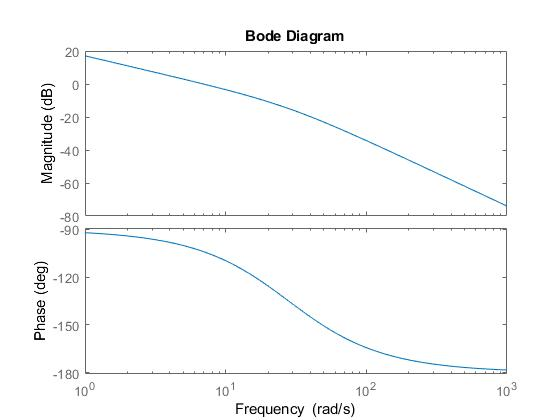
\includegraphics[width=0.8\textwidth]{./figures/lab2_theta.jpg}
	\caption{Bode plot for $\theta$ (Generated by MatLab)}
	\label{fig:}
\end{figure}

\begin{figure}[H]
	\centering
	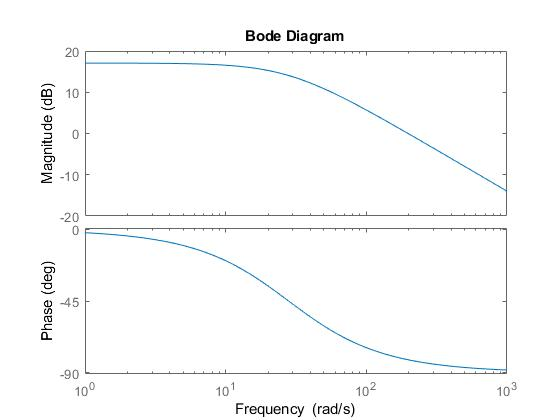
\includegraphics[width=0.8\textwidth]{./figures/lab2_omega.jpg}
	\caption{Bode plot for $\omega$ (Generated by MatLab)}
	\label{fig:}
\end{figure}

\section{Angular Position \& Velocity Plots}

\begin{figure}[H]
	\centering
	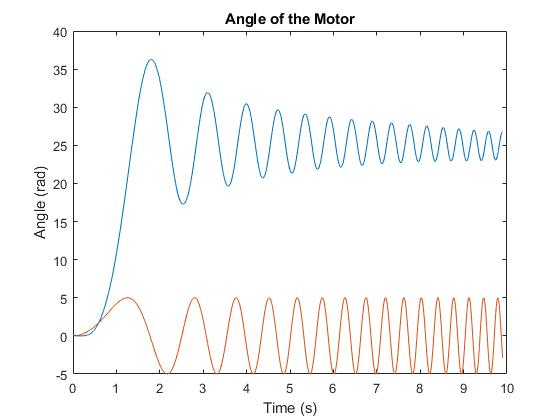
\includegraphics[width=0.8\textwidth]{./figures/lab2_theta_with_input.jpg}
	\caption{Motor Angular Position}
	\label{fig:}
\end{figure}

\begin{figure}[H]
	\centering
	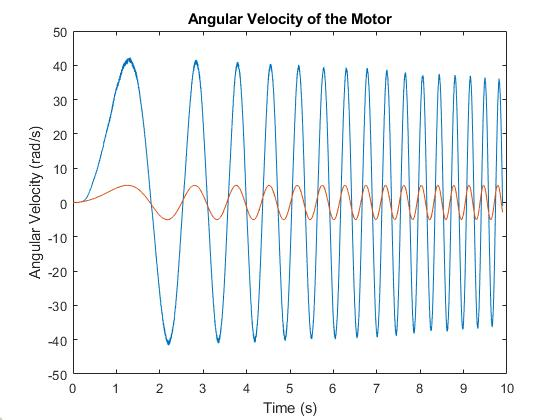
\includegraphics[width=0.8\textwidth]{./figures/lab2_omega_with_input.jpg}
	\caption{Motor Velocity}
	\label{fig:}
\end{figure}

For the plot of $\omega$, as the frequency increased, the amplitude stayed constant for a while and then began to slowly decrease, which matches the Bode plot. For the phase angle both sinusodes began at a phase angle of 0 degrees. As the frequency increased, the phase angle appears to decrease over time, but we could not quantify this difference because our test ended. 

For the plot of $\theta$, as frequency increased the amplitude decreased, which was predicted by the Bode plot. At very low frequencies, the amplitude tended towards very large values. The phase angle origin began at a trough, which signifies a phase angle of -90 degrees, while the other one began at a phase angle of 0, both predictions following along with our Bode plots.  

\subsection{Tabulated Data}

\begin{table}[H]
	\centering
	\caption{Data Collection Table}
	\label{tab:data-collection}
	\begin{tabular}{|| c c c c c c ||}
		\hline
		$\omega$ & Magnitude & Gain (dB) & Zero-Time Difference & Phase (rad) & Phase (deg) \\ [0.5ex]
		\hline\hline
		0.5 & 7.2805 & 17.2433 & 0.2364 & 0.1182 & -6.7726 \\
		\hline
		0.7896 & 6.9883 & 16.8875 & 0.0467 & 0.0368 & -2.1106 \\
		\hline 
		1.2469 & 7.037 & 16.3012 & -0.0597 & 0.0745 & 4.2661 \\
		\hline 
		1.9692 & 7.2075 & 17.1557 & 0.0183 & 0.0361 & -2.0663 \\
		\hline
		3.1098 & 6.9883 & 16.8875 & 0.0509 & 0.1582 & -9.0661 \\
		\hline
		4.911 & 6.8666 & 16.7348 & -0.0079 & -0.00386 & 2.2102 \\
		\hline 
		7.7554 & 6.5501 & 16.3249 & 0.0295 & 0.2285 & -13.0901 \\
		\hline 
		12.2474 & 5.99 & 15.5486 & 0.0317 & 0.3888 & -22.2763 \\
		\hline 
		19.3413 & 5.3813 & 14.6177 & 0.0268 & 0.5181 & -29.6827 \\
		\hline 
		30.5439 & 4.6751 & 13.3959 & 0.00206 & 0.6284 & -36.0026 \\
		\hline 
		48.2352 & 3.0924 & 9.8059 & 0.0174 & 0.841 & -48.1836 \\
		\hline 
		76.1734 & 3.0924 & 9.8059 & 0.0114 & 0.8668 & -49.6612 \\
		\hline 
		120.2936 & 2.3132 & 7.2843 & 0.0089 & 1.0757 & -61.6309 \\
		\hline 
		189.9696 & 1.7288 & 4.755 & 0.0077 & 1.4687 & -84.1504 \\
		\hline 
		300 & 1.534 & 3.7167 & 0.0068 & 2.0292 & -116.2648 \\
		\hline 
	\end{tabular}
\end{table}

\subsection{Experimental Bode Plots}

\begin{figure}[H]
	\centering
	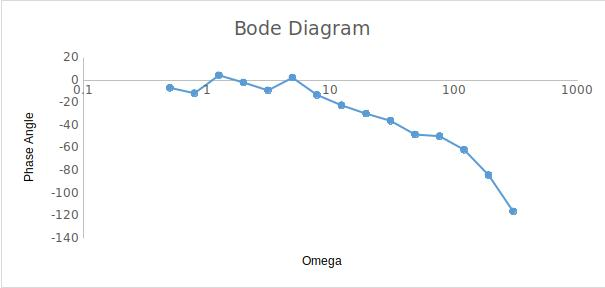
\includegraphics[width=0.8\textwidth]{./figures/lab2_experiment_phase.jpg}
	\caption{Experimental bode plot for phase angle}
	\label{fig:}
\end{figure}

\begin{figure}[H]
	\centering
	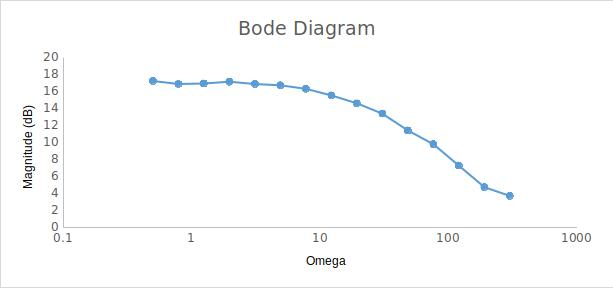
\includegraphics[width=0.8\textwidth]{./figures/lab2_experiment_magnitude.jpg}
	\caption{}
	\label{fig:}
\end{figure}

    % \lecture{4}{Tue 04 Feb 2020 14:30}{393 Lab 4}

\section{Plots of System response varying $\omega_{0}$, $\zeta$}
The result of varying $\zeta$ is the graph in Figure \ref{fig:varying-zeta}.
\begin{figure}[H]
	\centering
	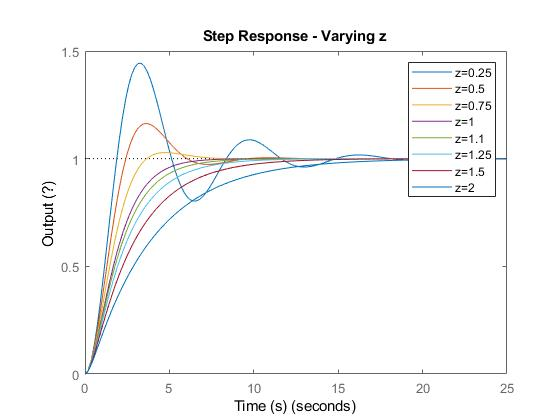
\includegraphics[width=0.8\textwidth]{./figures/lab4_fig1-part4-3-1-z.jpg}
	\caption{A plot of the system response when varying the value of $\zeta$}
	\label{fig:varying-zeta}
\end{figure}
As you can see an increase in $\zeta$ increases the damping of the output, where $\zeta=1$ seems to be close to the critical damping value, $\zeta < 1$ is an underdamped system and $\zeta > 1$ is an overdamped system. 

The result of varying $\omega_{0}$ is seen in Figure \ref{fig:varying-w0}.
\begin{figure}[H]
	\centering
	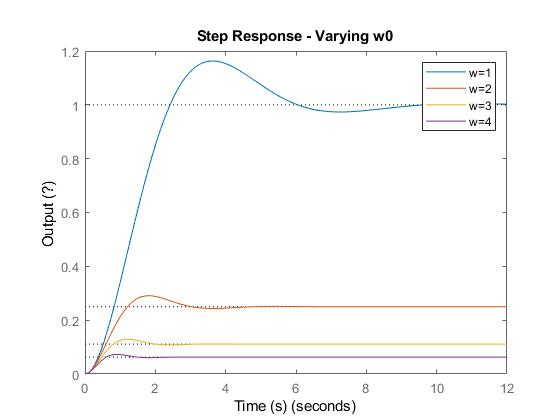
\includegraphics[width=0.8\textwidth]{./figures/lab4_fig2-part4-3-1-w0.jpg}
	\caption{A plot of the system response when varying the value of $\omega _{0}$}
	\label{fig:varying-w0}
\end{figure}
The greater the value of $\omega_{0}$, the smaller the steady-state value of the system. 

\section{Effects of Changing $\alpha$}  %Maxym
For positive values of $\alpha$, the effect of increasing $\alpha$ is the graph in Figure \ref{fig:varying-alpha-positive}.
\begin{figure}[H]
	\centering
	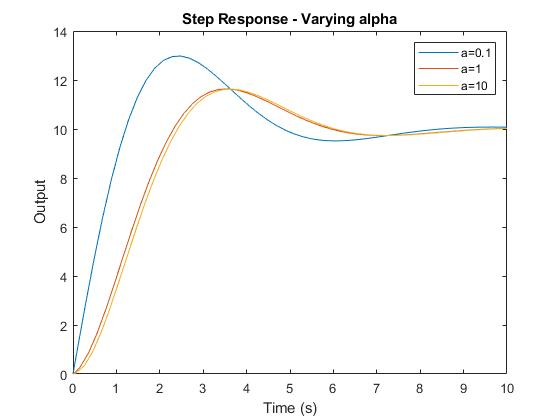
\includegraphics[width=0.8\textwidth]{./figures/lab4_fig3-part4-3-2-positive.jpg}
	\caption{A plot of the system response when varying the positive values of $\alpha$}
	\label{fig:varying-alpha-positive}
\end{figure}
As $\alpha$ increases, the rise time of the system also increases. While there is a large difference between the rise times of $\alpha = 0.1$ and $\alpha = 1$, the difference between $\alpha = 1$ and $\alpha = 10$ is relatively small. Meanwhile, settling time for all positive values of $\alpha$ appear relatively similar with all of the values converging to 10 at approximately 10 seconds. All three positive values of $\alpha$ displayed overshoot with $\alpha = 0.1$ having the largest overshoot while $\alpha =1$ and $\alpha = 10$ had smaller overshoots. Similarly, the peak time of $\alpha = 0.1$ is much shorter than the peak times of $\alpha = 1$ and $\alpha = 10$. The graph shows that $\alpha = 10$ has the longest peak time. 

For negative values of $\alpha$, the effect of increasing $\alpha$ is the graph in Figure \ref{fig:varying-alpha-negative}.
\begin{figure}[H]
	\centering
	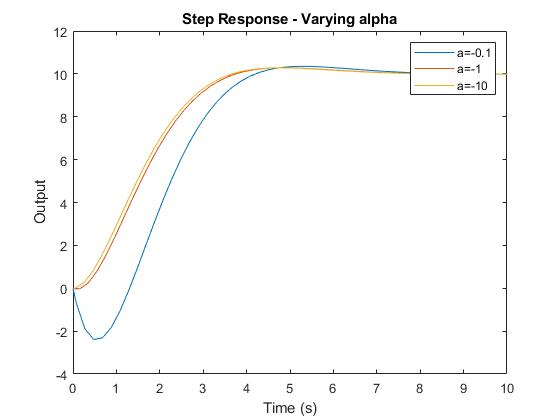
\includegraphics[width=0.8\textwidth]{./figures/lab4_fig4-part4-3-2-negative.jpg}
	\caption{A plot of the system response when varying the negative value of $\alpha$}
	\label{fig:varying-alpha-negative}
\end{figure}
As $\alpha$ increases negatively, the rise time of the system decreases. While there is a large difference between the rise times of $\alpha = -0.1$ and $\alpha = -1$, the difference between $\alpha = -1$ and $\alpha = -10$ is relatively small. Meanwhile, settling time for all negative values of $\alpha$ appear relatively similar with all of the values converging to 10 at just under 10 seconds. All three negative values of $\alpha$ displayed small overshoot with $\alpha = -0.1$ having a slightly larger overshoot than $\alpha =1$ and $\alpha = 10$. The peak time of $\alpha = -0.1$ is slightly longer than the peak times of $\alpha = 1$ and $\alpha = 10$ which had similar peak times.
% End Maxym Section

\section{Why Are The Plots The Same?}
\begin{figure}[H]
        \centering
        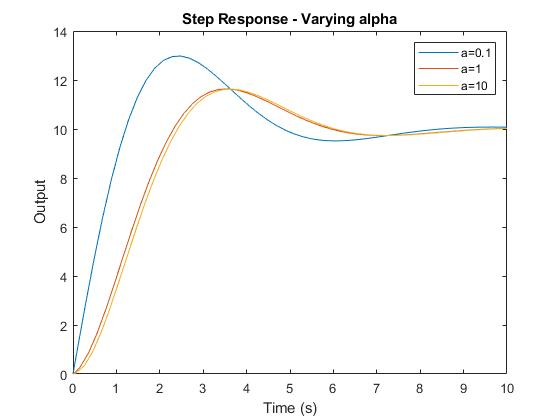
\includegraphics[width=0.8\textwidth]{./figures/lab4_fig3-part4-3-2-positive.jpg} % Put the plots in the figures sub     directory
        \caption{A one-sentence description of the plot or figure}
        \label{fig:name} % basically a variable name you can refer to in the text 
\end{figure}

\begin{figure}[H]
        \centering
        \includegraphics[width=0.8\textwidth]{./figures/lab4_fig3-part4-3-2-negative.jpg} % Put the plots in the figures sub     directory
        \caption{A one-sentence description of the plot or figure}
        \label{fig:name} % basically a variable name you can refer to in the text 
\end{figure}

\section{System Type Section}

\begin{table}[h]
\begin{tabular}{|l|l|l|l|l|}
System & \begin{tabular}[c]{@{}l@{}}Response to \\ Constant Input\end{tabular}                    & \begin{tabular}[c]{@{}l@{}}Response to \\ Linear Input\end{tabular}                      & \begin{tabular}[c]{@{}l@{}}Response to \\ Quadratic Input\end{tabular}                  & Type \\ \hline
1      & \begin{tabular}[c]{@{}l@{}}Settling Time 0.4s\\ Steady Error \textless 0.01\end{tabular} & \begin{tabular}[c]{@{}l@{}}Settling Time 0.4s\\ Steady Error \textless 0.08\end{tabular} & \begin{tabular}[c]{@{}l@{}}Settling Time 0.4s\\ Steady Error \textless 0.1\end{tabular} & 1    \\
2      & \begin{tabular}[c]{@{}l@{}}No Steady State\\ Error was Sinusoidal\end{tabular}           & \begin{tabular}[c]{@{}l@{}}No Steady State\\ Error was Sinusoidal\end{tabular}           & \begin{tabular}[c]{@{}l@{}}No Steady State\\ Error was Sinusoidal\end{tabular}          & 0    \\
3      & \begin{tabular}[c]{@{}l@{}}Settling Time 0.7s\\ Steady Error 8.5\end{tabular}            & \begin{tabular}[c]{@{}l@{}}No Steady State\\ Error was Linear\end{tabular}               & \begin{tabular}[c]{@{}l@{}}No Steady State\\ Error was Quadratic\end{tabular}           & 0
\end{tabular}
\end{table}

With a proportional control of \(P = 5\), the response tracked constant input \ref{fig:system1_constant}, linear input \ref{fig:system1_linear}, and constant input \ref{fig:system1_quadratic} all with a rise time of approximately \(0.4 s\) and steady state error of \(< 0.1\) in all cases. However, in the case of linear and quadratic input, the signal did not stabilize within a small error margin of the input signal and the error was not steady, which matches with the prediction that this is a type 1 system.

With a integral control of \(I = 1\), the response did not track any input, and the error was sinusoidal and increasing, or not BIBO stable in all cases. The response is graphed in the constant case \ref{fig:system2_constant}, linear \ref{fig:system2_linear}, and quadratic \ref{fig:system2_quadratic} This aligns with our predictions that System 2 is a Type 0 system.

With a derivative control of \(D = 1\), the response reached a steady state response with constant input \ref{fig:system3_constant}, but with a very large steady state error of \(8.5\) after \(0.7 s\). In the linear \ref{fig:system3_linear} and quadratic \ref{fig:system3_quadratic} cases, the steady state error was linear and quadratic respectively, and increasing. No steady state was reached, and the constant steady state was not acceptable, which agrees with our predictions that System 3 is a Type 0 system.

\begin{figure}[H]
        \centering
        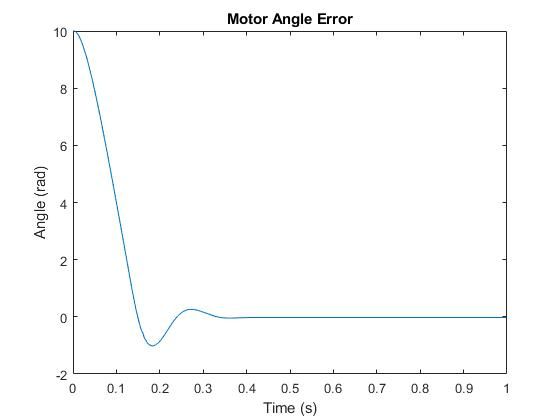
\includegraphics[width=0.8\textwidth]{./figures/lab4_fig7-part4-3-3-error-rc5.jpg}
        \caption{System 1 Response to Constant Input}
        \label{fig:system1_constant}
\end{figure}

\begin{figure}[H]
        \centering
        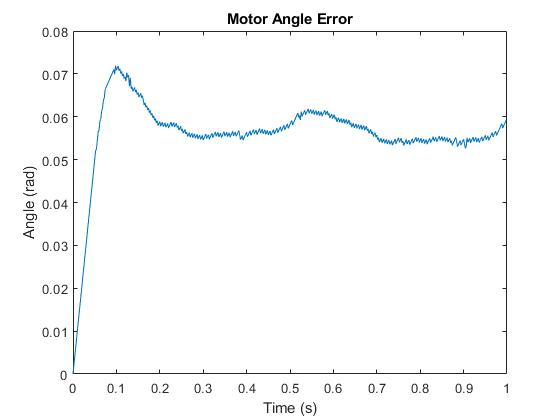
\includegraphics[width=0.8\textwidth]{./figures/lab4_fig8-part4-3-3-error-rc5-linear.jpg}
        \caption{System 1 Response to Linear Input}
        \label{fig:system1_linear}
\end{figure}

\begin{figure}[H]
        \centering
        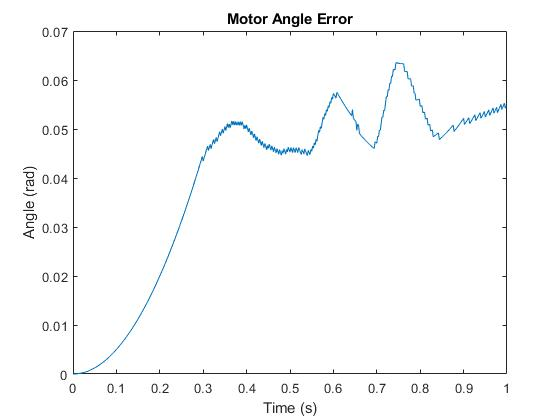
\includegraphics[width=0.8\textwidth]{./figures/lab4_fig9-part4-3-3-error-rc5-quadratic.jpg}
        \caption{System 1 Response to Quadratic Input}
        \label{fig:system1_quadratic}
\end{figure}

\begin{figure}[H]
        \centering
        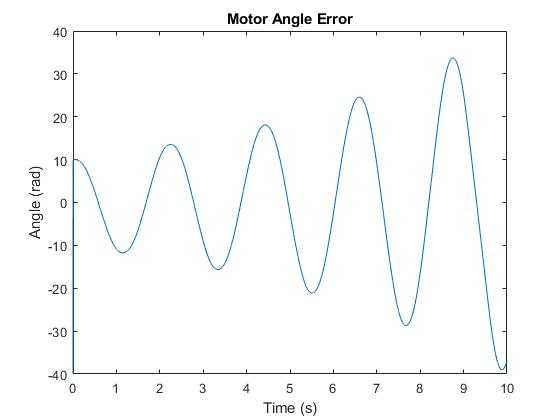
\includegraphics[width=0.8\textwidth]{./figures/lab4_fig10-part4-3-3-error-rc-I=1-constant.jpg}
        \caption{System 2 Response to Constant Input}
        \label{fig:system2_constant}
\end{figure}

\begin{figure}[H]
        \centering
        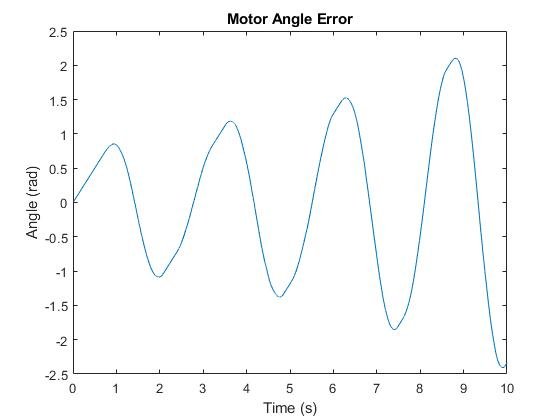
\includegraphics[width=0.8\textwidth]{./figures/lab4_fig11-part4-3-3-error-rc-I=1-linear.jpg}
        \caption{System 2 Response to Linear Input}
        \label{fig:system2_linear}
\end{figure}

\begin{figure}[H]
        \centering
        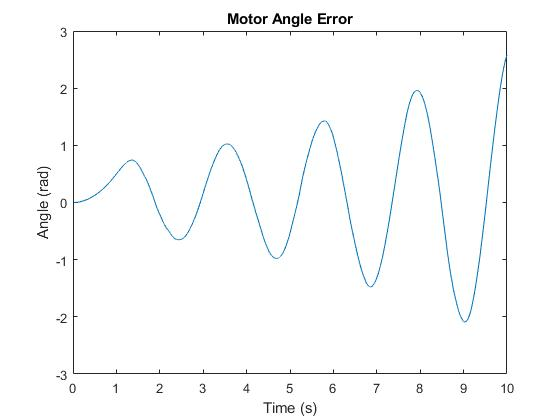
\includegraphics[width=0.8\textwidth]{./figures/lab4_fig12-part4-3-3-error-rc-I=1-quadratic.jpg}
        \caption{System 2 Response to Quadratic Input}
        \label{fig:system2_quadratic}
\end{figure}

\begin{figure}[H]
        \centering
        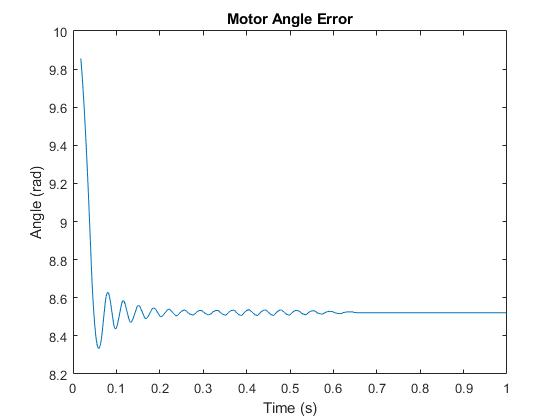
\includegraphics[width=0.8\textwidth]{./figures/lab4_fig13-part4-3-3-error-rc-D=1-constant.jpg}
        \caption{System 3 Response to Constant Input}
        \label{fig:system3_constant}
\end{figure}

\begin{figure}[H]
        \centering
        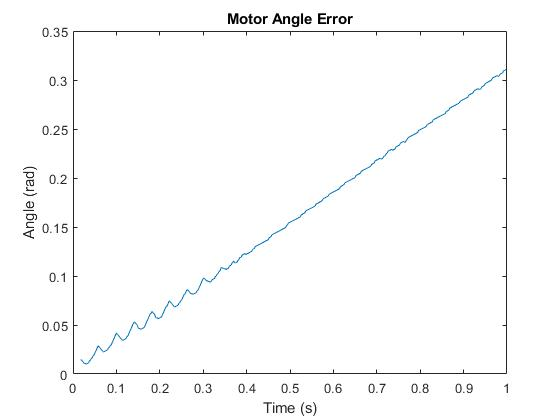
\includegraphics[width=0.8\textwidth]{./figures/lab4_fig14-part4-3-3-error-rc-D=1-linear.jpg}
        \caption{System 3 Response to Linear Input}
        \label{fig:system3_linear}
\end{figure}

\begin{figure}[H]
        \centering
        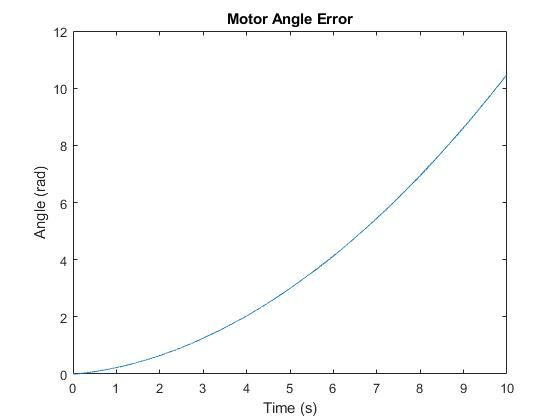
\includegraphics[width=0.8\textwidth]{./figures/lab4_fig15-part4-3-3-error-rc-D=1-quadratic.jpg}
        \caption{System 3 Response to Quadratic Input}
        \label{fig:system3_quadratic}
\end{figure}

    \lecture{5}{Tue 14 Jan 2020 10:26}{Addendum to guest lecture}

\begin{remark}[Limits of $x_{i}$ in the Multivariate Hypergeometric distribution]
	The constraints that Michael (guest lecturer) wrote are: 
	\begin{align*}
		x_1 + \ldots+ x_{r} &=  k \\
		max(0, k - \left( N - n_i \right) ) &\le x_{i} \le min\left( n_{i}, k \right) \\
		i &= 1, \ldots, r
	.\end{align*}
	There is an additional constraint: $x_{i} $ is an integer, $i = 1, \ldots, r$.

	Alternatively, we can set the constraints to be 
	\begin{align*}
		x_1 + \ldots + x_r &= k \\
		x_{i} &\in  \left\{ 0, 1, \ldots, n_{i} \right\} , i = 1, \ldots, r
	.\end{align*}
\end{remark}

An alternative way to describe the distribution of $\left( X_1, \ldots, X_{r} \right) $ is to describe the distribution of $\left( X_1, \ldots, X_{r-1} \right) $ and use the constraint $X_1 + \ldots + X_{r} = k$. 

We have:
\begin{align*}
	P\left( X_1 = x_1, \ldots, X_{r-1} = x_{r-1} \right) &= P\left( X_1= x_1, \ldots, 
	X_{r-1} = x_{r-1}, X_r = k - x_1-\ldots-x_{r-1} \right)  \\
							     &=\frac{\binom{n_1}{x_1} \binom{n_2}{x_2} \cdots \binom{n_{r-1}}{x_{r-1}}  \binom{n_{r}}{k-x_1-\ldots-x_{r-1}}}{\binom{N}{k}}
.\end{align*}
for:
\begin{align*}
	0 &\le x_1 + \ldots + x_{r-1} \le k \\
	x_i &= 0, \ldots, n_{i} \\
	max&\left( 0, k-\left( N - n_{i} \right)  \right) \le x_{i}\\
	i &= 1, \ldots, r-1 
.\end{align*}
We can write the marginal distribution of $\left( X_{i_{i}}, \ldots, X_{i_{d}} \right) $, $\left\{ i_{1}, \ldots, i_{d} \right\}  \subset \left\{ 1, \ldots, r \right\} $ by relabelling the objects in the population as types $i_{1}, \ldots, i_{d}$,and "other". 

There are $N - n_{i_{1}} - \ldots - n_{i_{d}}$ objects of type other.

Using the second version of the Multivariate Hypergeometric distribution, we have that the joint pmf of $\left( X_{i_{1}}, \ldots, X_{i_{d}} \right) $ is 
\begin{align*}
	P\left( X_{i_{1}}= x_{i_{1}}, \ldots, X_{i_{d}} = x_{i_{d}} \right) 
	&= \frac{\binom{n_{i_{1}}}{x_{i_{1}}}  \cdots \binom{n_{i_{d}}}{x_{i_{d}}}  \binom{N - n_{i_{1}} - \ldots - n _{i_{d}}}{k-x_{i_{1}}-\ldots-x_{i_{d}}}}{\binom{N}{k}}
 \\
	0 \le x_{i_{1}} + \ldots + x_{i_{d}} &\le  k \quad x_{ij} = 0, \ldots, n_{i_{j}}\\
	max\left( 0, k- \left( N - n_{ij} \right)  \right) &\le x_{ij}, \quad j = 1, \ldots, d
.\end{align*}

    \lecture{6}{Fri 17 Jan 2020 15:55}{}

Last time: $\hat{F} : \T \times X  \to \R^{n}$ 

Solution: $\dot{\xi} \left( t \right) = \hat{F}\left( t, \xi \left( t \right)  \right) $, almost everywhere $t \in  \T' \subseteq \T$. 

Domain:
\[
D_{\hat{F}} = \left\{ \left( t, t_0, x_0 \right) \in \T\times \T\times X \\
\mid \text{ solution exists at time }t, w \text{ initial conclusion }x_0 \text{ at initial time } t_0\right\} 
.\] 

Flow: $\Phi ^{\hat{F}} : D_{\hat{F}} \to X$ satisfies 
\[
	\frac{d}{dt}\Phi ^{\hat{F}}\left( t, t_0, x_0 \right)  = \hat{F}\left( t, \Phi ^{\hat{F}}\left( t, t_0, x_0 \right)  \right) , \quad \Phi ^{\hat{F}}\left( t_0, t_0, x_0 \right)  = x_0
.\] 
\begin{example}
	$\T = \R$, $X = \R$, $\hat{F}\left( t, x \right) = x^2$. Solution with initial condition $x_0$ at time $t_0$ satisfies 
	\begin{align*}
		\dot{\xi }\left( t \right)  &=  \xi \left( t \right) ^2 \\
		\xi \left( t_0 \right) &= x_0 \\
		\dot{x} &= x^2 \\
		\frac{dx}{x^2} &= dt \\
		\implies x\left( t \right) &= \frac{x_0}{1 - x_0\left( t - t_0 \right) } 
	.\end{align*}

	\[
		D_{\hat{F}} = \left\{ \left( t, t_0, x_0 \right)  \mid \begin{cases}
				t \in \left( -\infty, t_0 + \frac{1}{x_0} \right) & x_0 > 0 \\
				t \in  \left( t_0 + \frac{1}{x_0}, \infty \right) & x_0 < 0 \\
				t \in  \left( -\infty, \infty \right)  & x = 0
		\end{cases} \right\} 
	.\] 
	\begin{align*}
		\Phi ^{\hat{F}}: D_{\hat{F}} &\longrightarrow \R \\
		\left( t, t_0, x_0 \right)  &\longmapsto \Phi ^{\hat{F}}(\left( t, t_0, x_0 \right) ) = \frac{x_0}{1 - x_0\left( t - t_0 \right) }
	.\end{align*}
\end{example}

For linear equations, there are no restrictions on the times for which solutions exist.
\[
\implies D_{\hat{F}} = \T \times  \T \times  X 
.\] 

\subsection{Autonomous ODE's (independent of time)}

An ODE $\hat{F} : \T \times  R  \to \R ^{n} $ is autonomous if $\exists  \hat{F}_{0} : X  \to \R^{n}$ so that $\hat{F}\left( t, x \right) = \hat{F} _{0}\left( x \right) $. This just captures the idea of independence of time. 

    \lecture{7}{Mon 20 Jan 2020 08:39}{Marginal CDF's}

\begin{definition}
	Let $X_1, \ldots, X_{n}$ have joint cdf $F_{x}\left( x_1, \ldots, x_{n} \right)  = P \left( X_{1} \le x_1, \ldots, X_{n}\le x_{n} \right) $. 

	Let $\left\{ i_1, \ldots, i_{k} \right\} \subset \left\{ 1,\ldots,n \right\} $ and 
	\[
	\left\{ j_1, \ldots, j_{n-k} \right\} = \left\{ 1, \ldots, n \right\} \ \left\{ i_1, \ldots, i_{k} \right\} 
	.\] 
	where $i_1, \ldots, i_{k}$ are distinct. 

	The joint marginal CDF of  $\left( X_{i_1} ,\ldots, X_{i_{k}} \right) $ is 
	\begin{align*}
		F_{X_{i_1}, \ldots, X_{i_{k}}}\left( x_{i_{1}}, \ldots, x_{i_{k}} \right) 
		&= P\left( X_{i_{1}} \le  x_{i_{1}}, \ldots, X_{i_{k}} \le  x _{i_{k}} \right) \\ 
		&= P\left( X_{i_{1}} \le  x_{i_{i}} ,\ldots, X_{i_{k}} \le X_{i_{k}} \le x_{i_{k}}, \
		X_{j_{1}} < \infty, \ldots, X _{j_{n-k}} < \infty \right)  \\
	        &=  \lim_{x_{j_{1}} \to \infty, \ldots , x_{j_{n - k}} \to \infty} P\left( X_{i_{1}} \le  x_{i_{i}} ,\ldots, X_{i_{k}} \le X_{i_{k}} \le x_{i_{k}}, X_{j_{1}} < \infty, \ldots, X _{j_{n-k}} < \infty \right) 
	.\end{align*}

	In other words, take the full joint CDF and let elements $j_1, \ldots, j_{n - k} \to \infty$. 
\end{definition}

\section{Independence of Multiple Random Variables}

First, let us look at $n$ events $A_1, \ldots, A_{n}$. What do we mean for them to be mutually independent?

For $n = 2$: Intuitively (and mathematically), we want $P\left( A_1  \mid A_2\right) = P\left( A_1 \right) $ where $P\left( A_1 \mid A_2 \right) $ is the conditional probability of $A_1$ given $A_2$. 

\begin{figure}[ht]
    \centering
    \incfig{venn-diagram-of-$-and-$}
    \caption{Venn Diagram of $A_{1}$ and $A_2$}
    \label{fig:venn-diagram-of-$-and-$ }
\end{figure}

In the new probability space above, the crossed lines implies that $A_1$ happened given $A_2$ occurred. Then
 \[
	 P\left( A_1 \mid A_2 \right)  = \frac{P\left( A_1 \cap A_2 \right) }{P\left( A_2 \right) }
.\]
So if $A_1$ and $A_2$ are independent, then we have 
\begin{align*}
	\frac{P\left( A_1 \cap A_2 \right) }{P\left( A_2 \right) } &= P\left( A_1 \right)  \\
	\implies P\left( A_1 \cap A_2 \right)  &= P\left( A_1 \right) P\left(A_2 \right) 
.\end{align*}

Now consider n events $A_1, \ldots, A_n$.

\begin{definition}
	$A_1, \ldots, A_{n}$ are mutually independent if 
	\begin{align*}
		P\left( A_1\cap \ldots \cap A_{n} \right) &= P\left( A_1 \right) \times \ldots \times P\left( A_{n} \right) \\
	P\left( A_{i_{1}}\cap \ldots\cap A_{i_{k}}\right)  &= P\left( A_{i_1} \right) \times  \ldots \times  P\left( A_{i_{k}} \right) \quad \forall \left\{i_1,\ldots, i_{k} \right\} \subset  \left\{ 1, \ldots, n \right\} 
	.\end{align*}
\end{definition}
\begin{remark}
	Pairwise independence $\not\implies$  mutual independence. 
	\begin{example}
		Three 
	\end{example}
\end{remark}

    \lecture{8}{Tue 21 Jan 2020 10:35}{Independence of Random Variables}

\begin{definition}
	We say that $n$ random variables $X_{1} , \ldots , X_{n}$ are mutually independent if 
	\[
		P\left( X_1 \in A_1, \ldots, X_{n} \in  A_{n} \right) = P\left( X_1 \in  A_1 \right) \times \ldots\times P\left( X_{n}\in A_{n} \right) 
	.\] 
	for any $A_{1} , \ldots , A_{n} \subset \R$ (any reasonable set).

	Note that we can take any of the $A_{i}$ to be $\R$, so if we take $\left\{ i_{1} , \ldots , i_{k} \right\} \subset \left\{ 1, \ldots , n \right\} $ and $\left\{ j_{1} , \ldots , j_{n-k} \right\}  = \left\{ 1, \ldots, n \right\}  \ \left\{ i_{1} , \ldots , i_{k} \right\} $ , then
	\begin{align*}
		P\left( X_{i_{j}} \in A_{i_{1}}, \ldots, X_{i_{k}} \in  A_{i_{k}} \right) &= P\left( X_{i_{1}} \in  A_{i_1}, \ldots, X_{i_{k}} \in A_{i_{k}}, X_{j_1} \in  A_{j_1} \in  \R, \ldots, X_{j_{n-k}} \in \R \right)  \\
											  &= P\left( X_{i_1} \in A_{i_1} \right) \ldots P\left( X_{i_{k}} \in  A_{i_{k}} \right) \left( 1 \right) \ldots \left( 1 \right)  \\
											  &= P\left( X_{i_1} \in A_{i_1} \right) \ldots P\left( X_{i_{k}} \in  A_{i_{k}} \right) 
	.\end{align*}
	So any subset of $X_{1} , \ldots , X_{n}$ are mutually independent if $X_{1} , \ldots , X_{n}$ are mutually independent. 
\end{definition}

\begin{remark}
	 \begin{enumerate}
		 \item If $X_{1} , \ldots , X_{n}$ are mutually independent then so are $g_{i}\left( X_1	 \right) , \ldots , g_{n}\left( X_{n} \right) $ where $g_{i} : \R \to \R, i = 1, \ldots, n$.
		 \item The $X^{ir}_{i}$ in the definition of independence can be any random quantities (eg, random vectors or random matrices). The only change is that the $A^{is}_{i}$ must be in the appropriate range space of $X_{i}$. 
	\end{enumerate}
\end{remark}

\begin{theorem}
	$X_{1} , \ldots , X_{n}$ are mutually independent if and only if $f_{x}\left( x_{1} , \ldots , x_{n} \right) = f_{X_{1}}\left( x_1 \right) \times  \ldots\times f_{X_{n}}\left( x_{n} \right) $ (cts case with marginal pdfs) or 
	 \[
		 P_{X}\left( x_{1} , \ldots , x_{n} \right) = P_{X_{1}}\left( x_1 \right) \times \ldots\times P_{X_{n}}\left( x_{n} \right) 
	.\] 
	(discrete case with marginal pmfs).

\begin{proof}
	Suppose the above factoring holds. Let $A_{1} , \ldots , A_{n}\subset \R$ be arbitrary. Then
	\begin{align*}
		P\left( X_1 \in  A_1, \ldots, X_{n} \in  A_{n} \right) &= \begin{cases}
			\int_{A_{n}}^{ } \ldots \int_{A_1}^{ } dx_{1} , \ldots , dx_{n}  & \text{continuous} \\
			\sum_{X_{n} \in  A_{n}}^{ } \ldots \sum_{x_1 \in  A_{n}}^{ }  P_{X}\left( x_{1} , \ldots , x_{n} \right) & \text{discrete}
		\end{cases}\\
		&= \begin{cases}
			\left( \int_{A_{n}}^{ } f_{X_{n}}\left(x_{n}\right) dx_{n} \right) 	\times \ldots\times \left( \int_{A_{1}}^{ } f_{X_{1}}\left(x_{1}\right) dx_{n} \right) \\
			\left( \sum_{x_{n} \in  A_{N}}^{ } P_{X_{n}}\left( x_{n} \right)  \right) \times  \ldots \times \left( \sum_{x_1 \in  A_1}^{ } P_{X_1}\left( x_1 \right)  \right) 
		\end{cases} \\
		&= P\left( X_{n} \in  A_{n} \right) \times \ldots\times P\left( X_1 \in  A_1 \right) 
	.\end{align*}
	Now assume that $X_{1} , \ldots , X_{n}$ are mutually independent:
	\begin{description}
		\item[Discrete Case] By independence
			\begin{align*}
				P\left( X_{1} = x_1, \ldots, X_{n} = x_{n}\right) &= P\left( X_1 = x_1 \right) \times \ldots\times P\left( X_{n} = x_{n} \right)  \\
				\implies P_{X}\left( x_{1} , \ldots , x_{n} \right) &= P_{X_1}\left( x_1 \right) \times \ldots\times P_{X_{n}}\left( x_{n} \right) 
			.\end{align*}
	\end{description}
\end{proof}
\end{theorem}

    \lecture{9}{Thu 23 Jan 2020 09:36}{Expectation and Multiple RVs}

\begin{theorem}
	$X_{1} , \ldots , X_{n}$ are mutually independent if and only if  
	\[
		F_X \left( x_{1} , \ldots , x_{n} \right) = F_{X_1} \left( x_1 \right) \times \ldots \times F_{X_{n}} \left( x_{n} \right) 
	.\] 
	where $F_{X}$ is joint cdf and $F_{X_{i}}$ is marginal cdf of $X_{i}$, $i = 1, \ldots, n$. 
	\begin{proof}
		Suppose $X_{1} , \ldots , X_{n}$are mutually independent. Then
		\begin{align*}
			F_{X}\left( x_{1} , \ldots , x_{n} \right) 
			&= P\left( X_1 \le x_1, \ldots, X_{n} \le  x_{n} \right)  \\
			&= P\left( X_1 \le x_1 \right)  \times \ldots\times  P\left( X_{n} \le x_{n} \right)  \\
			&= F_{X_1} \left( x_1 \right) \times \ldots\times F_{X_{n}}\left( x_{n} \right) 			
		.\end{align*}
		Now suppose that 
		\begin{align*}
			F_{X}\left( x_{1} , \ldots , x_{n} \right) &= F_{X_1} \left( x_1 \right) \times \ldots\times F_{X_{n}}\left( x_{n} \right) \quad \forall \left( x_{1} , \ldots , x_{n} \right) \in R^{n}
		.\end{align*}
		In this case when $X_{1} , \ldots , X_{n}$ are jointly continuous then from proof of previous theorem we get that $f_{X}\left( x_{1} , \ldots , x_{n} \right) = f_{X_1}\left( x_1 \right) \times \ldots\times f_{X_{n}}\left( x_{n} \right) $, which then implies that $X_{1} , \ldots , X_{n}$ are mutually independent.  
		
To prove that $F_{X}\left( x_{1} , \ldots , x_{n} \right) = F_{X_1}\left( x_1 \right) \times \ldots \times F_{X_{n}}\left( x_{n} \right) $ implies that $X_{1} , \ldots , X_{n}$ are mutually independent is outside of the scope of this course. 
	\end{proof}
\end{theorem}

\section{Expectation Involving Multiple Random Variables}

Expectation is only defined for random variables. If $X = \left( X_{1} , \ldots , X_{n} \right) ^{T}$ is a random vector then we may write $E\left[ X \right] $, which only means
\[
\begin{bmatrix} E\left[ X_1 \right] \\ \vdots\\ E\left[ X_n \right]  \end{bmatrix}
.\] 
Now, each $E\left[ X_{i} \right] $ is with respect to the marginal distribution of $X_{i}$. However, it is not necessary to compute each marginal distribution.

\begin{theorem}[Law of Unconscious Statistician]
	If $g\left( x_{1} , \ldots , x_{n} \right) : \R^{n} \to \R$ is a real valued function of $x_{1} , \ldots , x_{n}$, then
	\begin{align*}
		E\left[ g\left( X_{1} , \ldots , X_{n} \right)  \right] = \begin{cases}
			\int \ldots \int_{\R^{n}} g\left( x_{1} , \ldots , x_{n} \right)  f_{X}\left( x_{1} , \ldots , x_{n} \right) dx_{1} , \ldots , dx_{n} & \text{continuous} \\
			\sum_{x_{n}}^{ }  \ldots \sum_{x_1}^{ } g\left( x_{1} , \ldots , x_{n} \right) p_{X}\left( x_{1} , \ldots , x_{n} \right)  & \text{discrete}
		\end{cases}
	.\end{align*}
	\begin{proof}[Discrete Case]
		Let $Y = g\left( X_{1} , \ldots , X_{n} \right) $. Then 
		\begin{align*}
			E\left[ g\left( x_{1} , \ldots , x_{n} \right)  \right]  == E\left[ Y \right] \\
			&= \sum_{Y} y P\left( Y = y \right)  \\
			&= \sum_{y}^{ } y \sum_{x:g\left( x \right)  = y} P\left( X = x \right) , \quad x = ( x_{1} , \ldots , x_{n}) \\
			&= \sum_{y}^{ } \sum_{x: g\left( x \right) = y} g\left( x \right) P\left( X = x \right)  \\
			&=\sum_{x} g\left( x \right) P\left( X = x \right)
		.\end{align*}
	\end{proof}
\end{theorem}

\begin{example}
	Suppose $\left( X_1, X_2 ,X_3  \right) $ have joint pdf 
	\[
		f\left( x_1, x_2, x_3 \right) = \frac{1}{\sqrt{2 \pi} }e^{\frac{-\left( x_1 - x_3 \right) ^2}{2 }} \frac{1}{\sqrt{2 \pi} }e^{\frac{-\left( x_2 - x_3 \right) ^2}{2 }}  \frac{1}{\sqrt{2 \pi} }e^{\frac{- x_3  ^2}{2 }} 
	.\] 
	Compute $E\left[ X_1 X_2 \right] $. In our heads. 
	\begin{itemize}
		\item Integrate with respect to $x_1$ first - only present in one term. Pull everything else out of the integral.
		\item Same process with $x_2$. 
		\item Finally do the same with $x_{3}$. You're left with a normal $(0, 1)$ distribution. 
	\end{itemize}
\end{example}


    % end lectures
\end{document}
